\chapter{Zufallsvariablen}
\textbf{Definition}:\\
Eine ZV ist eine Funktion X:$\Omega$ $\rightarrow \mathbb{R}$\smallskip\\\textbf{Beispiel}:\\
2 Würfel. \hspace{1cm}$\Omega = \{(a_1,a_2): a_1,a_2 \in \{1,...,6\}\}$\medskip\\
Erste Augenzahl: $X_1(a_1,a_2)=a_1$\\
Zweite Augenzahl $X_2(a_1,a_2)=a_2$\\
Augensumme: $X(a_1,a_2) = a_1 + a_2 \qquad x = x_1 + x_2$\\
Größe Augenzahl: $y(a_1,a_2)=max(a_1,a_2)$\medskip\\
\textbf{In dieser Vorlesung sei $\Omega$ immer endlich}\medskip\\
\textbf{Definition}:\\
Eine Verteilung einer ZV X ist die Angabe der Werte und der Wahrscheinlichkeiten dieser Werte.\smallskip\\
	Zähldichte von X : $\Omega \rightarrow\mathbb{R}$ ist $P_x:\mathbb{R}\rightarrow[0,1]$\medskip
\begin{center}
	$P_x(t)=\mathds{P}\underbrace{[x = t]}_\text{Er.} = \mathds{P}[\underbrace{\{w \in \Omega:X(\omega)=t\}}_{x^{-1}(t)}]$\medskip\\
\end{center}
	
\textbf{Beispiel}: 2 Würfel. \hspace{1cm} $x(a_1,a_2) = a_1 + a_2$ Augensumme\medskip\\
\begin{tabular}{c|c|c|c|c|c|c|c|c|c|c|c|}
	t&2&3&4&5&6&7&8&9&10&11&12\\\hline
	$\mathds{P}[x=t]$&$\frac{1}{36}$&$\frac{2}{36}$&$\frac{3}{36}$&$\frac{4}{36}$&$\frac{5}{36}$&$\frac{6}{36}$&$\frac{5}{36}$&$\frac{4}{36}$&$\frac{3}{36}$&$\frac{2}{36}$&$\frac{1}{36}$
\end{tabular}\medskip\\
\{x=2\} = \{(1,1)\}\\
\{x=3\}=\{(1,2),(2,1)\}\\
\{x=4\} = \{(1,3),(3,1),(2,2)\}\\
...\medskip\\
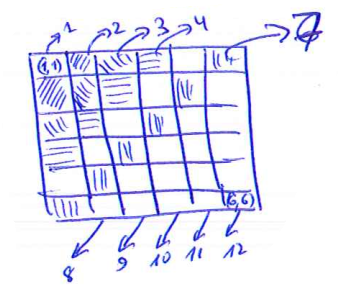
\includegraphics[width=0.4\textwidth]{img/okay.PNG}\\

\begin{math}
P_x(t)=
\begin{cases}
	\dfrac{t-1}{36}&, t \in \{2,...,7\}\medskip\\
	\dfrac{13-t}{36}& , t \in \{7,...,12\}\medskip\\
	0, t \notin \{2,...,12\}
\end{cases}
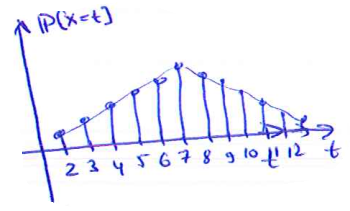
\includegraphics[width=0.4\textwidth]{img/diaa.PNG}\\
\end{math}\begin{floatingfigure}[r]{6cm}
	\mbox{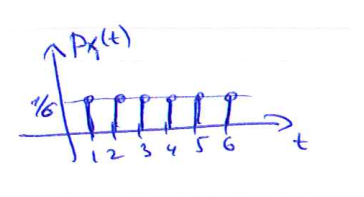
\includegraphics[width=0.4\textwidth]{img/dia.PNG}}
\end{floatingfigure}
Für die erste Augenzahl $x_1(a_1,a_2) = a_1$\medskip\\
\begin{tabular}{c|c|c|c|c|c|c}
	t&1&2&3&4&5&6\\\hline
	$\mathds{P[x_i = t]}$&$\frac{1}{6}$&$\frac{1}{6}$&$\frac{1}{6}$&$\frac{1}{6}$&$\frac{1}{6}$&$\frac{1}{6}$
\end{tabular}\\\\
\textbf{Eigenschaften der Zähldichte: }
\begin{enumerate}
	\item $P_x(t)\in [0,1]$
	\item $\sum_{t\in\mathbb{R}}P_x(t) = 1$
\end{enumerate}
\textbf{Beispiel}: Sei A $\subset$ $\Omega$\\
Indikatorvariable von A:\medskip\\
\begin{math}
\mathds{1}_A(\omega)=
\begin{cases}
1,& \omega \in A\\
0,& \omega \notin A
\end{cases}
\end{math}
\medskip\\
Grafik und Tabelle indikatorvariable\medskip\\
\textbf{Definition}: Sei X ZV mit Verteilung\medskip\\
\begin{tabular}{c|c|c|c|c}
	Werte&$y_1$&$y_2$&$y_3$&...\\\hline
	Wahrscheinlichkeiten&$P_1$&$P_2$&$P_3$&...
\end{tabular} \hspace{1cm}$\smallskip\\\mathds{P}[x = y_i] = p_i$\medskip\\
Erwartungswert von X ist $\mathds{E} X = \sum_i \underbrace{y_i}_\text{Werte} \underbrace{P_i}_\text{Wkeiten}$\medskip\\
\textbf{Beispiel}: 1 Würfel, $x_1$ Augenzahl\\
$\mathds{E}X_1 = 1*\frac{1}{6}+2*\frac{1}{6}+...+6*\frac{1}{6} = 3,5$\\
$\mathds{E}X$ ist \textbf{nicht} der wahrscheinlichste Wert: $\mathds{P} [X=3,5] = 0$\medskip\\
\textbf{Bemerkung:}\\
Betrachte $n=10^6$ Würfe. Augenzahlen: $X_1,X_2,...,X_n$\smallskip\\
Dann gilt $\dfrac{X_1+...+X_n}{n}\approx 3.5$\medskip\\
\textbf{Satz 9.1}$[\text{ alternative Formel für }\mathds{E}X]$\\
Sei $X:\Omega \rightarrow\mathbb{R}$. Dann gilt: 
$$\mathds{E}X = \sum_{\omega \in \Omega} X(\omega)\underbrace{\mathds{P}[\{\omega\}]}_{p(\omega)}$$
\textbf{Beweis}: Seien $y_1,...,y_m$ Werte von X\medskip\\
$A_1 = \{X = y_1\},\dots ,A_m=\{X=y_m\}$\smallskip\\
$A_i = \{\omega \in \Omega:X(\omega)=y_i$s\}\smallskip\\
$\Omega = A_i \dot\cup A_2\dot\cup \dots\dot\cup A_m$ ist disjunkte Zerlegung\smallskip\\
$\mathds{E}X \overset{\text{Def}}{=} \sum_i y_i*p_i = \sum_i y_i \mathds{P}[A_i]$\smallskip\\
$\sum_iy_i\sum_{\omega \in A_i} p(\omega) \overset{w \in A_i}{=}\sum_i \sum_{\omega \in A_i} X(\omega)p(\omega)$ \medskip\\
$	\Rightarrow X(\omega)=y_i$\medskip\\
\textbf{Satz 9.2}. Seien $x,y :\Omega \rightarrow\mathbb{R}$ Zufallsvariablen\smallskip\\
Dann gilt: $\mathds{E}[x+y] = \mathds{E}X+\mathds{E}y$\medskip\\
\textbf{Beweis}: \\
$\mathds{E}[x+y] \underset{9.1}{=} \sum_{\omega \in \Omega}(x+y)(\omega)*p(\omega)=$\smallskip\\
$=\sum_{\omega \in \Omega} (X(\omega)+y(\omega))p(\omega) = \sum_{\omega \in \Omega}X(\omega)*p(\omega)+\sum_{\omega \in \Omega}y(\omega)*p(\omega)\overset{9.1}{=}$\smallskip\\$\mathds{E}X+\mathds{E}y\qed$\medskip\\
\textbf{Bemerkung}: Allgemein: Für ZV $X_1,\dots,X_n : \Omega \rightarrow \mathbb{R}:\mathds{E}[X_1+\dots+X_n] =$\\$ \mathds{E}X_1+\dots+\mathds{E}X_n$\medskip\\
\textbf{Bemerkung}: Sei $X:\Omega \rightarrow \mathbb{R}, a\in \mathbb{R}, \mathds{E}[a*X]=a*\mathds{E}X$\medskip\\
\textbf{Beispiel}: n Würfel. Augenzahlen: $X_1,\dots,X_n$ \hspace{0.2cm} Augensumme: S=$X_1+\dots+X_n$
$$\mathds{E}S=\mathds{E}X_n+\ldots+ \underbrace{\mathds{E}X_n}_{=3,5} = n*3,5$$
\textbf{Beispiel}: Lotto 6 aus 49. (ohne Zurücklegen) Tippe auf \{1,\dots,6\} \\
Sei S die Anzahl der richtig geratenen Zahlen.\medskip\\
Werte von S: 0,1,\dots,6\smallskip\\
$\mathds{P}[S=k] = \dfrac{\binom{6}{k}*\binom{43}{6-k}}{\binom{49}{6}} $ , für k $\in$ \{0,\ldots,6\}\medskip\\
\begin{math}
S = X_1+\dots+X_6, \text{wobei }\medskip\\
X_i = 
\begin{cases}
1,&\text{falls Ball \textbf{i} gezogen wurde}\\
0,&\text{sonst}
\end{cases}\medskip\\
\mathds{E}S\underset{9.2}{=}\mathds{E}X_1+\dots+\mathds{E}X_6
\end{math}\medskip\\
\textbf{Bemerkung}:\medskip\\ $\mathds{E1}_A=$
\begin{tabular}{c|c}
	0&1\\\hline
	$1-\mathds{P}[A]$&$\mathds{P}[A]$
\end{tabular} = $\mathds{P}[A]$\newpage
\begin{math}
\mathds{E}X_i= \mathds{P}[\text{Ball \textbf{i} wurde gezogen}]\medskip\\
= \dfrac{\binom{48}{5}}{\binom{49}{6}}
=\dfrac{\left(\dfrac{48*47*46*45*44}{5!}\right)}{\left(\dfrac{48*47*46*45*44}{6!}\right)} = \dfrac{6!/5!}{49} = \dfrac{6}{49} \quad \forall i \in \{1,\dots,6\}\medskip\\
\mathds{E}S=\mathds{E}X_1+\dots\mathds{E}X_6=6*\dfrac{6}{49}=\dfrac{36}{49}
\end{math}\medskip\\
\textbf{Definition}:\\
Seien $X_1,\dots,X_n : \Omega \rightarrow\mathds{R}$ ZV\\
Sie heißen unabhängig, falls: 
$$\forall y_1,\dots,y_n \in \mathds{R}: \quad \mathds{P}[X_1 = y_1,X_2 =y_2,\dots,X_n=y_n]]$$
$$=\mathds{P}[X_1=y_1]*\dots*\mathds{P}[X_n]=y_n$$
\textbf{Bemerkung}: Sind $X_1,\dots,X_n$ unabhängig, dann gilt sogar:
$$\forall A_1,\dots,A_n \subset \mathds{R}: \mathds{P}[X_1 \in A_1,\dots,X_n \in A_n]$$
$$=\mathds{P}[X_1 \in A_1]*\dots*\mathds{P}[X_n \in A_n]$$\medskip\\
\textbf{Satz 9.3}:\\
Seien $X,Y :\Omega \rightarrow \mathds{R} $ \textbf{unabhängige} Zufallsvariablen\\
Dann gilt: $\mathds{E}[X*Y]= \mathds{E}X*\mathds{E}Y$\medskip\\
\textbf{2 Eigenschaften}:
\begin{enumerate}
	\item $\mathds{E}[x+y] = \mathds{E}x+\mathds{E}y \quad \forall x,y$
	\item $ \mathds{E}[x*y] = \mathds{E}x*\mathds{E}\text{$ y $ } \forall \text{unabh. } x,y$
\end{enumerate}
\textbf{Beweis}:\\
Notation:\\
Werte von X: 
\begin{tabular}{|c|c|c|}
	$x_1$&$x_2$&\dots\\\hline
	$p_1$&$p_2$&\dots
\end{tabular} \\
$\mathds{P}[X=x_i]=p_i$\smallskip\\
Werte von Y: 
\begin{tabular}{|c|c|c|}
	$y_1$&$y_2$&\dots\\\hline
	$q_1$&$q_2$&\dots
\end{tabular}\\
$\mathds{P}[Y=y_j]=p_j$\newpage
Betrachte Ereignisse: $A_{ij}=\{X=x_i, y=y_j\}\smallskip\\=\{\omega \in \Omega : X(\omega)=xi,y(\omega)=y_j\}$\medskip\\
\begin{center}
	\img{0.4}{tab}\\
\end{center}
$\Omega = \underset{i,j}{\dot\cup}A_{ij}$, d.h. $A_{ij}$ bilden disjunkte Zerlegung von $\Omega$\medskip\\
$\mathds{E}[x*y] \underset{9.1}{=} \sum_{\omega\in \Omega} p(\omega)*X(\omega)*Y(\omega)=$\medskip\\
$\sum_{i,j}\sum_{\omega\in A_{ij}} (p(\omega)*X(\omega)Y(\omega)x_iy_j)=$\medskip\\
=$\sum_{i,j}(x_iy_j\sum_{w\in A_{ij}})=\sum_{i,j}x_iy_j\mathds{P}[A_{ij}]$\medskip\\
$\mathds{P}[A_{ij}]=\mathds{P}[X=x_i, Y=y_j] \underset{\text{x,y unabh ZV}}{=} \mathds{P}[X=x_i]*\mathds{P}[Y=y_i]=p_i*q_j$\bigskip\\
$=\sum_{i,j}x_iy_jp_iq_j = \sum_{i,j}(x_ip_i)(y_jq_j)$\medskip\\
$=(\sum_ix_ip_i)(\sum_jy_jq_j) = \mathds{E}X*\mathds{E}Y \qed$\\\\
\textbf{Beispiel}: (zur Unabhängigkeit von Zufallsvariablen)\\
Betrachte n faire Würfel\smallskip\\
$X_i$ ist die Augenzahl, die der i-te Würfel zeigt\smallskip\\
 $\Omega$ = \{($a_1,...,a_n$)\} def $X_i(a_1,...,a_n) = a_i$\medskip\\
 \textbf{Behauptung 1}: Zufallsvariablen $X_1,\dots,X_n$ sind unabhängig\medskip\\
 \textbf{Beweis 1}:\\
 Z.z. $\mathds{P}[X_i = x_1,...,X_n=x_n] = \mathds{P}[X_i=x_i]*\dots\mathds{P}[X_n=x_n]$\medskip\\
$\{X_1 = x_1,\dots X_n = x_n\}=
\begin{cases}
(x_1,\dots,x_n), &\text{falls }\forall i:x_i \in \{1,...,6\}\\
\emptyset, & \text{falls } \exists i : x_i \notin \{1,...,6\}
\end{cases}$\smallskip\\
LS = $
\begin{cases}
\dfrac{1}{6^n},&\text{falls } \forall i: x_i \in \{x_i \in \{1,...,6\}\\
0,&\text{sonst}
\end{cases}$\\\\
RS: $\mathds{P}[X_1=x_1] = ?$\medskip\\
\{$X_1=x_1$\}=$\begin{cases}
\{(x_1,a_2,...,a_n):a_2,...,a_n \in \{1,\dots,6\}\}, &\text{falls }x_1 \in \{1,\dots,6\}\\
\emptyset, & \text{falls } \exists i : x_i \notin \{1,...,6\}
\end{cases}$\medskip\\
$\#\{X_1=x_i\}=\begin{cases}
6^{n-1},&\text{falls }x_1\in \{1,\dots,6\}\\
0,&\text{sonst}
\end{cases}$\medskip\\
$\mathds{P}[X_1=x_1]=\begin{cases}
\dfrac{6^{n-1}}{6^n},&\text{falls }x_1 \in \{1,\dots,6\}\\
0,&\text{sonst}
\end{cases}$\medskip\\
RS=$\begin{cases}
\dfrac{1}{6}*\dfrac{1}{6}*\dots\dfrac{1}{6} = \dfrac{1}{6^n},&\text{falls } \forall A_i : x_i \in \{1,\dots,6\}\\
0, & \exists i:x_i \notin \{1,\dots,6\}
\end{cases}$\\\\
LS = RS $\Rightarrow X_1,\dots,X_n$ unabh. ZV.\\\\
\textbf{Behauptung 2}: Sei S = $X_1 + \dots + X_n$ die Augensumme.\\
Dann sind $X_1$ und S abhängige Zufallsvariablen\medskip\\
\textbf{Beweis}: Z.z. $\exists$ a,b mit $\mathds{P}[X_1=a,S=b] \neq \mathds{P}[X_1=a]*\mathds{P}[S=b]$\\
Wir zeigen das für a =1, b=6*n\medskip\\
\textbf{LS}: $\mathds{P}[\underbrace{X_1=1,S=6n}_\text{Treten nicht gleichzeitig ein}] = 0$\smallskip\\
\textbf{RS}: $\mathds{P}[X_1 = 1] = \dfrac{1}{6}$\\$\mathds{P}[S=6n]=\dfrac{1}{6^n}$\medskip\\
RS = $\dfrac{1}{6}*\dfrac{1}{6^n} \neq 0$\medskip\\
LS $\neq$ RS $\Rightarrow$$X_1,S$ abh. \qed
 
